\documentclass[../thesis.tex]{subfiles}

\begin{document}

  \chapter{Experimental results}
  \label{ch:experimental-results}


    \section{Experimental approach}
    \label{sec:conducted-measurements}

        For the first time during the team's research on alumina membranes, systematic measurements were conducted. Due to the limited period of time, only some aspects of the membranes could be investigated in more detail. During the internship, I measured 25 membranes of 3 wafers using the experimental setup described in \cref{sec:experimental-setup}. \Cref{tbl:wafer-specifications} summarizes the main fefatures of these wafers.

        \subfile{tikz/wafers/membrane_distribution.tex}

        \begin{table}[tb]
          \caption{Wafer specifications. The wafers thickness $l_\mathrm{pore}$, floating time $t_\mathrm{float}$ of the \textit{barrier layer} dissolution process and pore diameter dispersion $\Delta d_\mathrm{pore}^\mathrm{MEB}$ measured by electron beam microscopy are noted. The latter two parameters apply to the open pore membranes of the respective wafer.}
          \label{tbl:wafer-specifications}
          \selectfontsize{10pt}
          \begin{tabu} {X[r]X[r]X[r]X[r]}
            \unitoprule \\
            \textbf{Wafer} & \textbf{$l_\mathrm{pore}$ $[\si{\micro\meter}]$} & \textbf{$t_\mathrm{float}$ $[\si{\minute}]$} & \textbf{$\Delta d_\mathrm{pore}^\mathrm{MEB}$ $[\si{\nano\meter}]$} \\
            \unimidrule \\
            292 &60  &36+4   &- \\
            294 &60  &33   &-  \\
            295 &30  &35 (38 for b)  &7  \\
            296 &60  &40  &-  \\
            \unitoprule \\
          \end{tabu}
        \end{table}
        \medskip

        Victor Doebele's inital measurements previous to this internship had already shown strong dispersions in the properties of the membranes of different wafers, but also within the same wafer. Therefore, my goal was to perform systematic measurements on alumina membranes to determine the source of these dispersions. To probe a possible dependency on the position of the membranes on the wafers, the labeling is done according to the convention shown in \cref{fig:membrane-distribution}.

        Due to the limited period of time, I chose to focus on the production step of the \textit{barrier layer} dissolution (compare \cref{subsec:barrier-layer-dissolution}) and the pore diameter reduction by atomic layer deposition. During the intership, I measured 25 membranes of 4 wafers using the experimental setup described in \cref{sec:experimental-setup}. \Cref{tbl:wafer-specifications} summarizes the main characteristics of these wafers. A processing scheme for the wafers 295 and 296, which also marks the conducted measurements, is given by \cref{fig:wafer-processing-plans}.
        \medskip

        \subfile{tikz/wafers/wafer_processing_plans.tex}


    \section{Membrane structure analysis}

      \subsection{Isotherm of an open pore membrane}
      \label{subsec:open-pore-isotherm}

        \Cref{fig:295b-open-pores} shows a typical isotherm obtained from the measurements of an open pore membrane (in this case membrane 296b'). The dependence of the liquid fraction $LF$ on the relative vapor pressure $P_\mathrm{rel}$ follows the behaviour expected for a porous material: The membrane fills at a pressure
        \begin{equation*}
          P_\mathrm{cond}^\mathrm{296b'}<P_\mathrm{sv}
        \end{equation*}
        and empties at an even lower pressure
        \begin{equation*}
            P_\mathrm{evap}^\mathrm{296b'}<P_\mathrm{cond}^\mathrm{296b'}<P_\mathrm{sv},
        \end{equation*}
        hereby displaying a hysteretic cycle. By the model of condensation and evaporation in an open pore, which was introduced in \cref{eq:cond-evap-non-ideal-pore}, a condensation at spinodal pressure $P_\mathrm{sp}$ and evaporation at equilibrium pressure $P_\mathrm{eq}$, with
        \begin{equation*}
          P_\mathrm{eq}<P_\mathrm{sp}<P_\mathrm{sv},
        \end{equation*}
        are expected. This is coherent with the observations as the shape of the volumetric isotherm qualitatively matches the theoretical loop displayed in \cref{fig:open-pore-loops}.

        For the tranmission measurement, two drops corresponding to the condensation and the evaporation are observed, as expected according to \cref{sec:scattering-in-alumina-membranes}. Moreover, higher transmission is observed for the filled state of the membrane than for the empty state. This is also coherent with the theory of index matching mentioned in \cref{sec:scattering-in-alumina-membranes}.
        \medskip

        The dashed lines in \cref{fig:295b-open-pores} mark the average condensation and evaporation pressures of the isotherm. For their determination, the steepest point of the liquid fraction graph is sought, which corresponds to the minima of the transmission signals as expected. Converting these to diameters using the \textsc{Kelvin} equations \cref{eq:p-sp} and \cref{eq:p-eq} yields
        \begin{align*}
          d_\mathrm{pore}^\mathrm{296b'}(P_\mathrm{rel,sp}^\mathrm{296b'}=0,956)=\SI{44,4}{\nano\meter}, \\
          d_\mathrm{pore}^\mathrm{296b'}(P_\mathrm{rel,eq}^\mathrm{296b'}=0,925)=\SI{51,3}{\nano\meter},
        \end{align*}
        which makes for results within the range of expeceted pore diameters. Furthermore, the transmission behaves according to theory in regard of the filled transmission in filled state being stronger than for the empty state.  (COMPARE TO SEM OF 296e???)
        \medskip

        \subfile{tikz/graphs/open_pore/296b_op.tex}

        \begin{figure}[p]
          \centering
          \subfloat[]{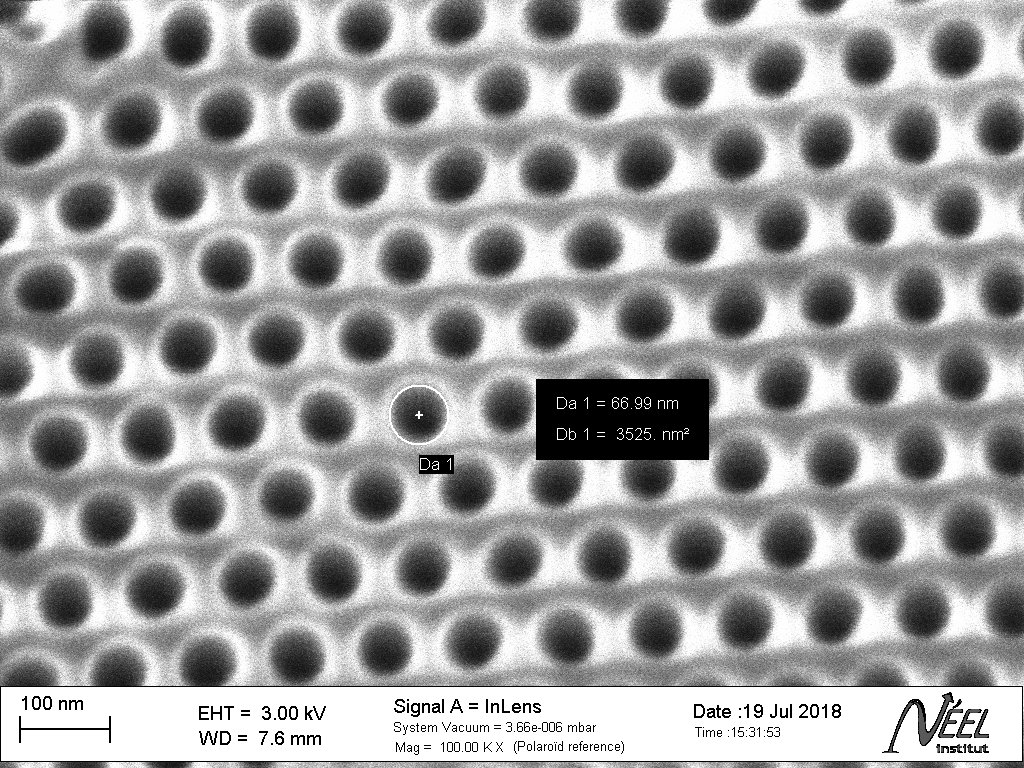
\includegraphics[width=.9\textwidth]{images/295g_pores_sol_side.jpg}
          \label{fig:295g-sol-side-sem}}
          \\
          \subfloat[]{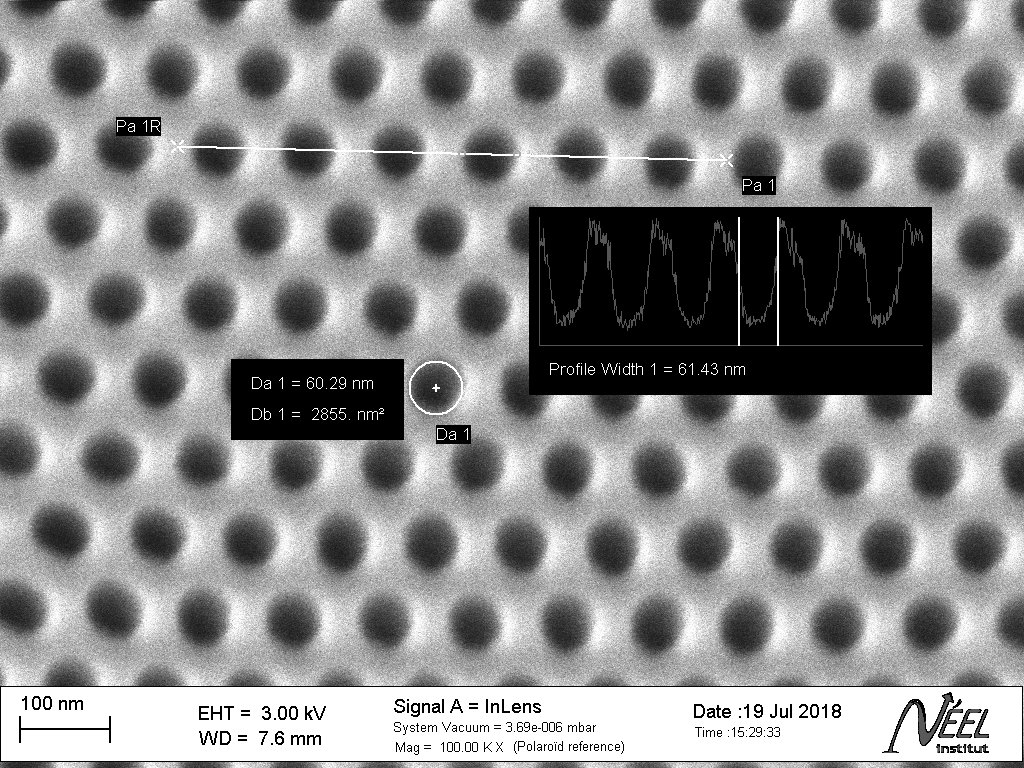
\includegraphics[width=.9\textwidth]{images/295g_pores_al_side.jpg}
          \label{fig:295g-al-side-sem}}
          \caption{SEM images of membrane 295g' implying the pores' funnellization. The pores on the solution side \protect\subref{fig:295g-sol-side-sem} show bigger diameters than those on the aluminum side \protect\subref{fig:295g-al-side-sem}.}
          \label{fig:295g-sem-funnellization-proof}
        \end{figure}

        However, if all the pores were cylindrical, the condensation and evaporation branches would be expected to be vertical. The inclination of evaporation branch could result from funnellization of the pores as has been explained in \cref{subsec:open-funnelled-pore-theory}. The SEM images of the membranes support the assumption of funnelled pores as different pore diameters are observed for the top and  bottom side (please refer to \cref{fig:295g-sem-funnellization-proof} for an example).  The condensation at spinodal pressure should still be vertical for weak funnelled pores, though. On the other hand, condensation at spinodal pressure in weakly funnelled cylindrical pores (compare \cref{subsec:open-funnelled-pore-theory}). This leads to the conclusion, that the pores are not only funnelled, but also distributed in diameter.



    \subsection{Isotherm of a closed pore membrane}
    \label{subsec:closed-pore-isotherm}

        \subfile{tikz/graphs/closed_pore_isotherm/cp_isotherm.tex}

        \Cref{fig:295b-closed-pores} shows the isotherm obtained on the same membrane 296b, but prior to the \textit{barrier layer} dissolution step. The open pore membrane's isotherm is also displayed for the sake of comparison. The results show that the hysteresis cycle is much smaller for closed pores than it has been observed for open pores. In detail, the condensation branch is shifted to much lower pressures, while the evaporation branch shows only a slight shift in the same direction.

        As will be explained in \cref{sec:opening-problem}, a small shift to lower pressures for the closed pore membrane is expected due to the widening of the pores during the \textit{barrier layer} dissolution process. Since, according to \cref{subsec:closed-funnelled-pore-theory}, the condensation occurs at equilibrium pressure in a closed pore, the smaller hysteresis of membrane 296b in comparison to 296b' is expected. However, as displayed in \cref{fig:closed-pore-loops}, the volumetric isotherm of a closed pore membrane should not show a hysteresis at all, not for straight pores and neither for funnelled pores. Its presence can be explained by variations of the pore diameters along the pores' lengths. These variations are so called \textit{corrugations}. The phenomenom of the hysteresis appearing for closed pores has been observed and accounted to corrugations by various experimentators (REF???).
        \medskip

        As for the transmission, the drops correspond to the condensation and evporation branch and also the effect of index matching is observed as expected from \cref{sec:scattering-in-alumina-membranes}. What remains to be understood is the extreme difference in magnitude between the transmission drops of the closed pore and the open pore membrane. In this magnitude, the phenomenom has only been observed for this specific membrane 296b so it might also be due to a light source within the experimental room that has not been turned off. As the membrane has been further processed, the measurement cannot be repeated though.


    \subsection{Measurement reproducibility}
    \label{subsec:measurement-reproducibility}

        \subfile{tikz/graphs/292c/292c_repro.tex}

        To check the reproducibility of the isotherm measurements, membranes were measured several times. \Cref{fig:292c-repro} shows four consecutive measurements for the same open pore membrane 292c and one more independent measurement ($LF_\mathrm{cond/evap}^\mathrm{292c,5}$). The biggest experiment deviation is the liquid fraction before the sharp rise of the condensation branch. However, this does not affect the position of the condensation and the evaporation rises, which are used to determine the pores' diameters.
        \medskip

        As at the time of these experiments the laser transmission setup had not been in place and later membranes were measured only two times at maximum, the reproducibility of the laser transmission measurements cannot be assesed here.


    \subsection{Inhomogeneities on one wafer}
    \label{subsec:wafer-inhomogeneities}

        \subfile{tikz/graphs/wafer_inhomogeneities/inhomogeneities_cp.tex}
        \subfile{tikz/graphs/wafer_inhomogeneities/inhomogeneities_op.tex}

        In this section, the isotherm measurements I performed in order to test the homogeneity of the wafers are presented for two production steps: The closed pore state after the aluminum dissolution process (compare \cref{subsec:al-dissolution}) in \cref{fig:inhomogeneities-cp} and the open pores after the \textit{barrier layer} dissolution (\cref{subsec:barrier-layer-dissolution}) in\cref{fig:inhomogeneities-op}.

        For both wafers the overall shapes of the different membranes' isotherm measurements matches. The only exception is the open pore membrane 295c', which will be discussed in ???. However, the results show that there is a dispersion on the condensation and evaporation branches. This implies a dispersion on the pore size distribution of about
        \begin{align*}
          \Delta d_\mathrm{closed-pore}^\mathrm{296} = \SI{3,5}{\nano\meter} \\
          \Delta d_\mathrm{closed-pore}^\mathrm{295} = \SI{4,7}{\nano\meter}
        \end{align*}
        for the closed pore membranes and
        \begin{align*}
          \Delta d_\mathrm{open-pore}^\mathrm{292} = \SI{4,1}{\nano\meter} \\
          \Delta d_\mathrm{open-pore}^\mathrm{295} = \SI{3,5}{\nano\meter}
        \end{align*}
        for the open pore membranes. The computations were done using the pressures of the top end of the widest spread evaporation branches of the respective wafer
        \begin{align*}
          P_\mathrm{evap,top}^\mathrm{296b}=0,9275,\quad P_\mathrm{evap,top}^\mathrm{296e'}=0,9225, \\
          P_\mathrm{evap,top}^\mathrm{295a}=0,9375,\quad P_\mathrm{evap,top}^\mathrm{295b}=0,9325, \\
          P_\mathrm{evap,top}^\mathrm{292c}=0,9275,\quad P_\mathrm{evap,top}^\mathrm{292d}=0,9325, \\
          P_\mathrm{evap,top}^\mathrm{295d'}=0,9430,\quad P_\mathrm{evap,top}^\mathrm{295e'}=0,9400,
        \end{align*}
        as these correspond to the emptying of the largest pores of a given membrane.
        \medskip

        Moreover, the transmission during the condensation and the evpoatiion of hexane within the membranes also shows dispersions across the wafers. \Cref{fig:wafer-transmission} shows color maps of the dry transmission of the membranes of the wafers 295 and 296. The membranes of wafer 296 have all been measured before any further treatments with phosphoric acid, whereas the membranes of wafer 295 are open pore membranes except for 295a and 295b, which are still closed. In comparison to the theoretical values computed using the \textsc{Fresnel} equations (compare \cref{eq:trans-coeffs}), the measured transmission coefficients are much smaller. This can be explained by the pores scattering light as explained in \cref{sec:scattering-in-alumina-membranes}. Talking wafer inhomogeneities, the measured transmission of membranes on the same wafer shows variations of up to $\SI{8}{\percent}$
        for the closed pore membrane of wafer 296 and $\SI{17}{\percent}$ for the open pore membranes of 295. A systematics regarding the the link between the pore diameters and the transmission value can be suspected when regarding the membranes 296a, 296b, 296e and 296f. For each pair of two neighboring membranes, the same transmission has been measured. The respective isotherms are displayed in \cref{fig:296-cp}. What strikes the eye is that the neighboring pores show almost perfectly superimposed volumetric isotherms, whereas the there is a clear shift in pressure between the two pairs' curves. To draw a conclusion, larger pore diameters (higher condensation pressures) go together with a stronger dry transmission. This conclusion has to be retested using other membranes as it has only been observed once.

        \subfile{tikz/wafers/transmission.tex}

        In conclusion, to measure the effect of treatments on a given membrane, before and after measurements are necessary. It is not enough to measure one membrane representatively for multiple membranes in the same state.


        \subsubsection{Transmission of open and closed pores}

          \Cref{fig:295-transmission} shows the measured dry transmission for the membranes of wafer 295. The membranes 295a and 295b are still closed pore membranes, while all other membranes have undergone the \textit{barrier layer} dissolution process opening their pores. Striking is the much better transmission of the closed pore membranes in comparison to the open pore membranes. Referring to the assumption made in \cref{subsec:wafer-inhomogeneities}, that larger pores cause stronger light scattering and therefore weaker transmission, the observed phenomenom could be explained by the increase of pore diameters upon the pore opening step. To verify this explanation, systematic experiments using the same open pore membrane and widening the pores by immersion in acid could be conducted.


    \subsection{Defects}
    \label{subsec:defects}

        All in all, the conducted measurements yield great results. The measured isotherms go along with the model introduced in \cref{eq:cond-evap-non-ideal-pore} and are reproducible. The inhomogeneity on a given wafer is bearable???.

        Nevertheless, pore defects and dispersions were detected. First, there is the pore size distribution. To estimate its broadness, SEM images are analyzed in 295g???. Next, the funnellization and the corrugation must be mentioned. Both cause intra pore diameter variations that cause inclined isotherms, even for a single pore. Last, bad open pores were detected during the measurements. This problem will be discussed in the following section, as its examination leads to valuable, relevant results.


  \section{The problem of pore opening}
  \label{sec:opening-problem}


      \subsection{Bad open pores}
      \label{subsec:bad-open-pores}

        \subfile{tikz/graphs/294_bad_open_pores/294_bad_open_pores.tex}

        Victor Doebele's measurements before my internship had revealed that the \textit{barrier layer} dissolution step failed to open all the pores of some membranes. The term \textit{bad open pores} refers to a membrane that has been floated on phosphoric acid for not long enough to completely open the pores. ???TIKZ IMAGE??? As a result some pores remain closed whereas others have constricted openings and some are fully open. \Cref{fig:294-bad-open-pores} shows the comparison of closed pore membrane 294cp and membrane 294op with bad open pores. The assumption is derived from the isotherm in the following way: By theory, the condensation branch should be shifted towards higher pressure for open pores in respect to closed pores. While this is the case for membrane 294op's end of the condensation rise, it still starts at the same pressure as the condensation of the closed pore membrane which by theory condenses at equilibrium pressure. Moreover, the evaporation of 294op is superimposed with the one of 294cp. While this is expected by theory, it rules out the possibility of an increase in funnellization or corrugation causing the broader condensation branch of the open pore membrane. The only possible explanation for the observed behaviour is a population of open pores alongside one of closed pores on the membrane. In this case some pores start filling at equilibrium pressure, wheras others fill at higher spinodal pressures depending on the size of the pore opening on the aluminum side. Independently, SEM images of the membrane confirm the assumption of bad open pores as shown in \cref{fig:294-sem}.

        \begin{figure}[p]
          \centering
          \subfloat[]{
          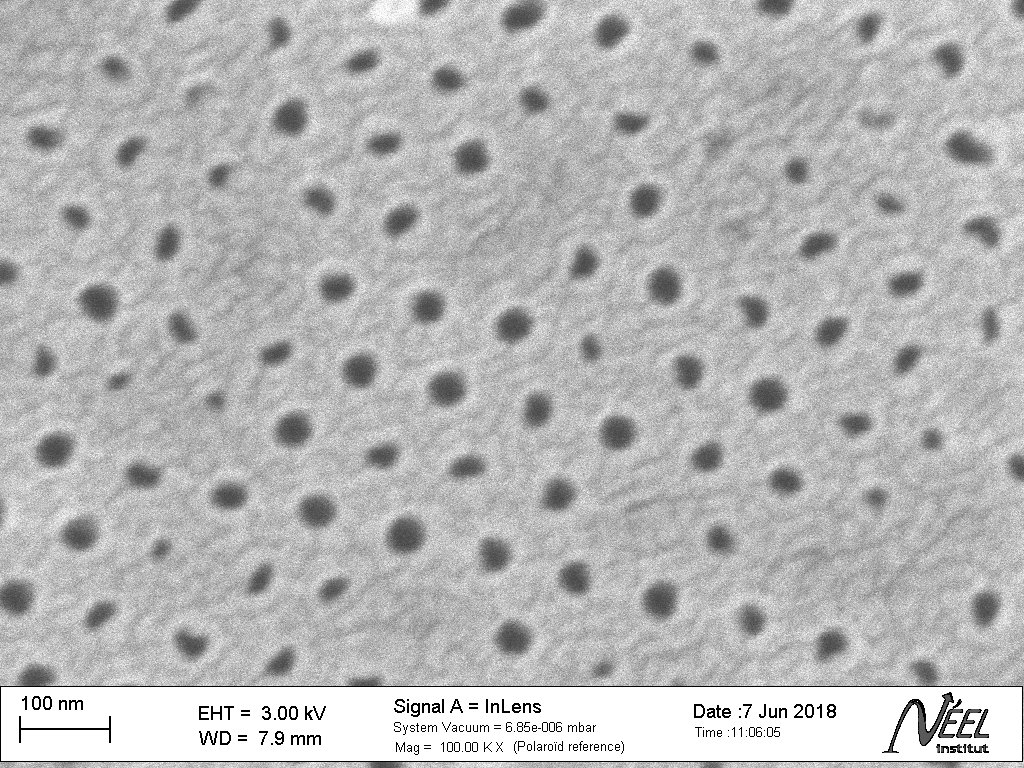
\includegraphics[width=0.9\textwidth]{images/294_bad_open_pores.jpg}
          \label{fig:294-sem}}  \\
          \subfloat[]{
          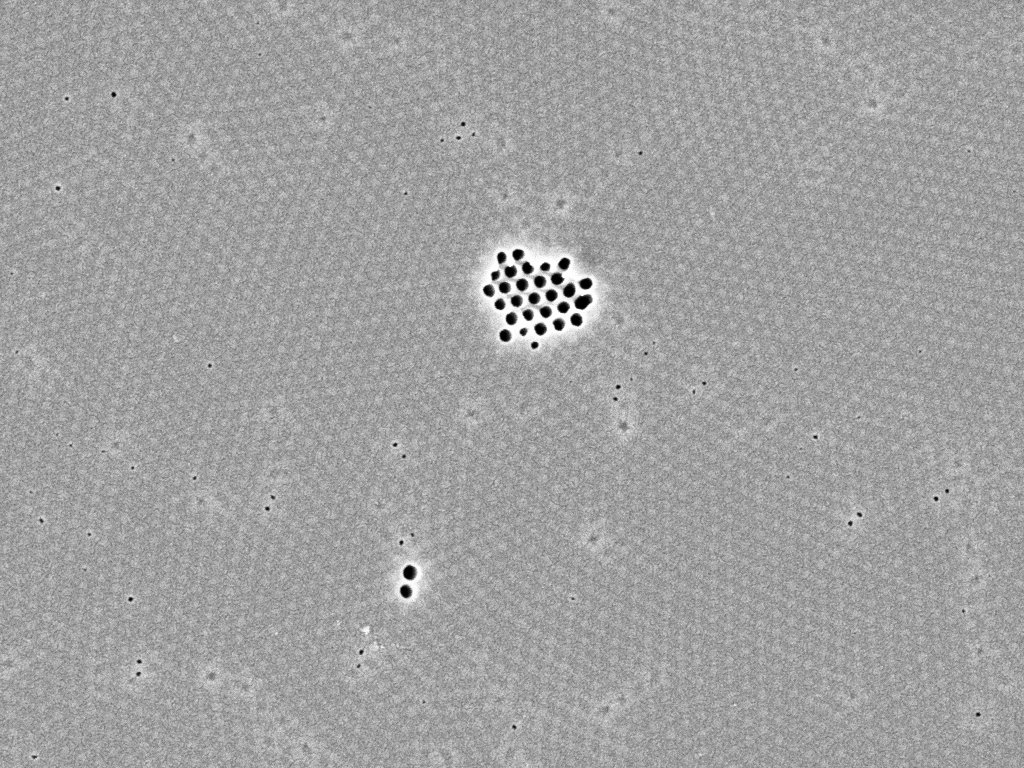
\includegraphics[width=0.9\textwidth]{images/sem_milky_etch.jpg}
          \label{fig:milky-meb}}
          \caption{\protect\subref{fig:294-sem} shows a SEM image confirming the bad open pores of membrane 294op. Image \protect\subref{fig:milky-meb} SEM image of a membran floated on phosphoric acid until the appearance of milky aspects. It is coherent with the link of the milky aspect to pores of a wafer starting to open.}
        \end{figure}

        At first glance, resolving the bad open pore issue seems as easy as simply increasing the membranes' floating time during the \textit{barrier layer} dissolution. On second thought though, a problem comes up: \Cref{fig:294-sem} clearly states that some pores open before others. Therefore, these open pores are infiltrated by phosphoric acid which starts etching the pore from the inside increasing its diameter. This results in a broadening pore diameter distribution on the membrane caused by the \textit{barrier layer} dissolution process.

        As mentioned in ???MEMBRANE PRODUCTION, milky aspects occur at some point of the floating. Same as for spinodal condensation in the membranes, the filling of the opening pores with acid is assumed to cause light scattering and can therfore be linked to these milky aspects. Proof of this theory is the SEM image taken of a membrane that has been floated until the milky aspects appeared. Shown in \cref{fig:milky-meb}, the image confirms the semi open state of the membrane. As the milky aspects last for about
        \begin{equation*}
          t_\mathrm{milky} =\SI{3}{\minute}
        \end{equation*}
        and the etch rate of phosphoric acid on alumina is expected to be
        \begin{equation*}
          e=\SI{1}{\nano\meter\per\second},
        \end{equation*}
        the \text{barrier layer} dissolution process should cause an increase of the pore diameter dispersion of
        \begin{equation*}
          \Delta d_\mathrm{pore} = \SI{6}{\nano\meter}.
        \end{equation*}
        This is quite dramatic regarding that the pore diameter distribution of a closed pore limited to about $\SI{10}{\nano\meter}$ ??? PROOVE!. Therefore, this increase should be obvious on the comparison of the evaporation branches of a closed pore membrane with an equivalent open pore membrane. Using \cref{fig:295b-closed-pores} as an example does not confirm these expectations. On the contrary, the evaporation branch seems to become more sharp by opening the pores. This leads to the suspicion that the etch rates parallel to the pore axis $e_\mathrm{\parallel pores}$ and perpendicular to the axis $e_\mathrm{\perp pores}$ are different. With the idea of using a combination of floating and immersion in phosphoric acid for the \textit{barrier layer} dissolution, an experiment to calibrate the etch rates has been conducted.
        \medskip

        Membranes of wafer 296 were floated and immersed in phosphoric acid for
        \begin{align*}
            \begin{split}
                t_\mathrm{im}^\mathrm{296c'}=\SI{6,5}{\minute}, \\
                t_\mathrm{im}^\mathrm{296d'}=\SI{13}{\minute},  \\
                t_\mathrm{fl}^\mathrm{296e'}=\SI{13}{\minute}, \\
                t_\mathrm{fl}^\mathrm{296f'}=\SI{26}{\minute},
            \end{split}
        \end{align*}
        where $t_\mathrm{im}^{i}$ are the immersion times and $t_\mathrm{fl}^{i}$ the floating times with $i\in \{ \mathrm{296c,296d,296e,296f}\}$. Assuming that the acid etches the \textit{barrier layer} at the same rate from within and outside the pores, these floating and immersion of the membranes 296c' and 296e' should yield the same reduction of the thickness, the same holds for the membranes 296d' and 296f'. At this point, the initial thickness of wafer 296 is assumed to be
        \begin{equation*}
          d_\mathrm{barrier-layer}^\mathrm{296} =\SI{30}{\nano\meter}
        \end{equation*}
        thick, same as for wafer 292. To probe the etch rate $e_\parallel$, SEM images are taken for all membranes after the treatment in phosphoric acid. These images also serve to measure the pore diameters on the solution side and hereby to calculate $e_\perp$. In addition, the pore diameters are checked using isotherm measurements.


        \subsection{Etch rate on the barrier layer}
        \label{subsec:etch-rate}

          \subfile{tikz/graphs/296_membranes/296_membranes.tex}

          \Cref{fig:barrier-layer-sems} shows the SEM images taken of the membranes 296c' and 296e' after immsersion and floating respectively. During the SEM session, a lot of drift and charging had to be dealt with which makes for a bad resolution of the images. However, what strikes the eye is the large thickness of the \textit{barrier layer}, even after the treatments with phosphoric acid, as it is still thicker than the inital thickness that has been assumed. In accordance with these SEM images, the isotherm comparison shown in \cref{fig:full-comp-w296} implies pores that are still closed on all four treated membranes. In explanation, the isotherms superimpose nicely with the untreated closed pore membrane 296a and also, the direct comparison to the open pore membrane 296b' reveals a strong shift of the condensation branch towards lower pressures. Bad open pores can be excluded by comparing to \cref{fig:294-bad-open-pores} and the corresponding explanations in \cref{subsec:bad-open-pores} (and from SEM images shown in appendix???).

          In conclusion, the anodization process (compare ???) does not yield the same \textit{barrier layer} thickness for different wafers, even using the same parameters. To conclude with, SEM images of one native membrane that has not undergone any treatments with phosphoric acid needs to be measure to get an idea of the intial \textit{barrier layer} thickness. If there are also dispersions of this thickness on one wafer remains to be probed.

          \begin{figure}[p]
            \centering
            \subfloat[]{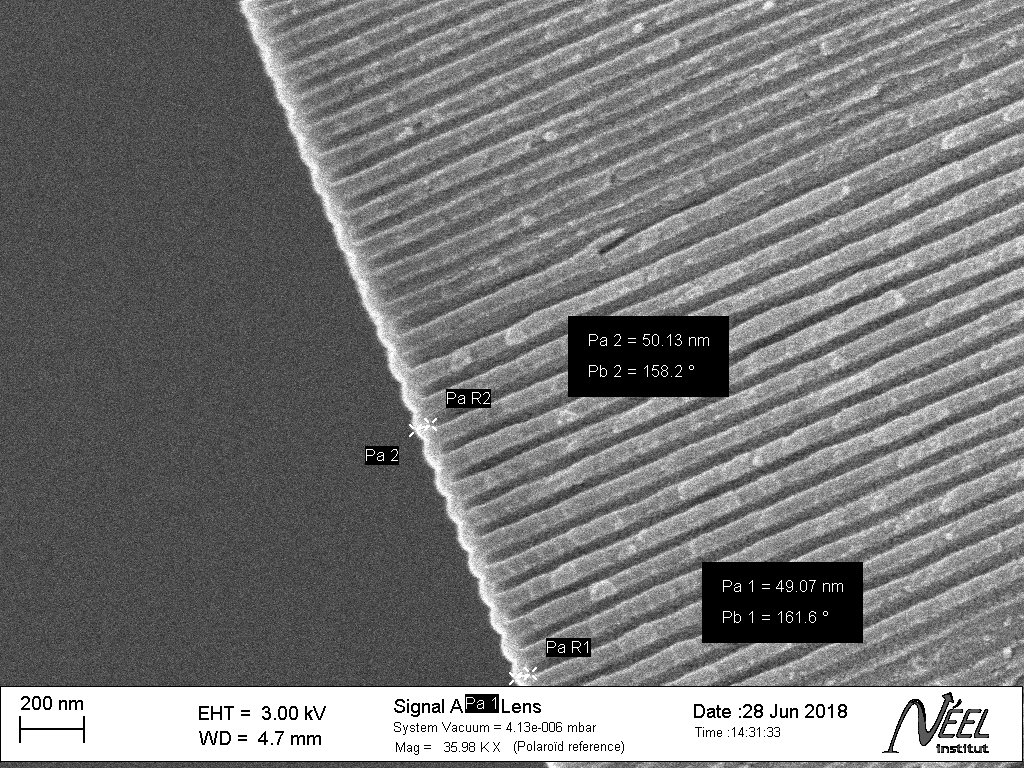
\includegraphics[width=0.9\textwidth]{images/296c_barrier_layer.jpg}
            \label{fig:296c-barrier-layer}} \\
            \subfloat[]{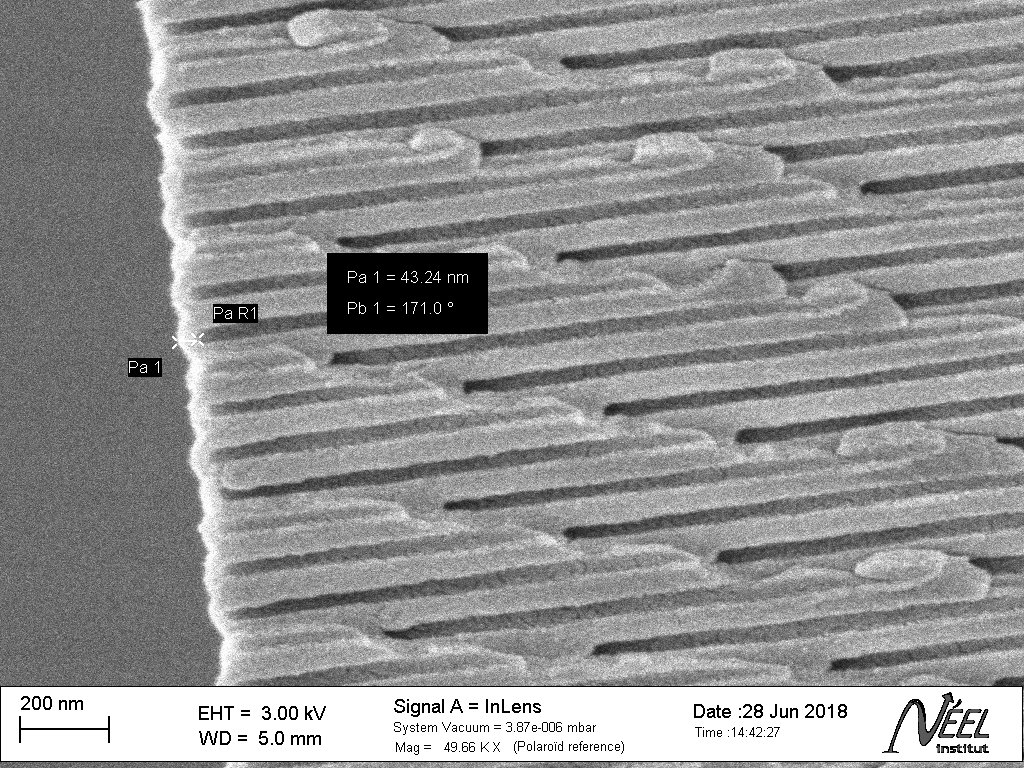
\includegraphics[width=0.9\textwidth]{images/296e_barrier_layer_meb.jpg}
            \label{fig:296e-barrier-layer}}
            \caption{SEM images with the aim to measure the thickness of the \textit{barrier layer} of the membranes 296c' and 296e'.}
            \label{fig:barrier-layer-sems}
          \end{figure}


        \subsection{Increase of funnellization upon immersion in phosphoric acid}
        \label{subsec:immersion-funnelling}

          \subfile{tikz/graphs/immersion_experiment/immersion.tex}

          The comparison of the immersed membranes 296c' and 296d' with the native membrane 296a yields a promising result. \Cref{fig:immersed-comp-w296} shows the three measured isotherms on a realtive vapor pressure axis revealing a shift of the top side of the evaporation rise to larger pressures going together with longer immersion times. At the same time, the bottom end of the condensation rise does not move to higher pressures. As it is closed pores that are dealt with (compare \cref{subsec:etch-rate}), the top end of the evaporation branch corresponds to the pore diameter at the top and, whereas the bottom end of the condensation branch corresponds to the diameter at the (smaller) closed end. Therefore, the observed phenomenom implies an etch rate that weakens along the pore axis towards the closed end. For further analysis of this acid saturation, \cref{fig:immersion-evap} and \cref{fig:immersion-cond} show \textsc{Kelvin} diameter conversions of the relevant pressure ranges. For the pressure isotherms, the evaporation rises have an exponential shape. Therefore, the converted diameter offset increases linearly along the liquid fraction which corresponds to the position in along the pore axis of a funnelled pore. The etch rate gradient along the pore length as plotted in \cref{fig:etch-rate-plot} can be derived from the values noted in \cref{tbl:etch-rate}. The corresponding shape evolution of a pore is illustrated in \cref{fig:funneling-increase}.

          At this point it is save to say that the phosphoric acid saturates within the pores due to the lack of circulation.

          \begin{table}[tb]
           \caption{Diameter reduction per minute of immersion derived from the isotherms of the membranes 296a, 296c, 296d.}
           \label{tbl:etch-rate}
           \selectfontsize{10pt}
           \begin{tabu} {X[r]X[r]X[r]}
             \unitoprule \\
             \textbf{$t_\mathrm{im} [\si{\minute}]$} & \textbf{$\Delta d_{h=\SI{60}{\micro\meter}} [\si{\nano\meter}]$} & \textbf{$\Delta d_{h=\SI{0}{\micro\meter}} [\si{\nano\meter}]$} \\
             \unimidrule \\
             0 &0  &0 \\
             6,5 &3  &0  \\
             13  &6  &0  \\
             \unitoprule \\
           \end{tabu}
          \end{table}

          \subfile{tikz/wafer_analysis/funnelling_increase.tex}


        \subsection{Inverse funnellization upon barrier layer dissolution}
        \label{subsec:inverse-funnelling}

          With the results of the immersion experiment explained above in \cref{subsec:inverse-funnelling}, the comparison of closed and open pore isotherms can be further analysed. \Cref{fig:op-cp-comp} shows two plots. Both compare the isotherm measured for a given membrane in closed state to the isotherm measured for the same membrane after the \textit{barrier layer} dissolution. This permits the comparison disregarding the intra wafer dispersions that were concluded in \cref{subsec:wafer-inhomogeneities}. The regarded membranes are 295b and 296b.

          \subfile{tikz/graphs/cp_op_comp/cp_op_comp.tex}

          For both membranes, the trend of the isotherm to sharpen is clearly visible. Regarding the funnellization, the evaporation branch is of special interest. That it straightens upon the pore opening step implies that the funnellization decreases. Referring to the saturation of phosphoric acid within the pores upon immersion concluded in \cref{subsec:immersion-funnelling}, the inverse funnellization can be explained as follows: During the \textit{barrier layer} dissolution the pores begin to open when the milky aspects appear. When they have disappeared, one might think the pores are open. But after having measure the bad open pores of wafer 294, Laurent Cagnon waits for another $\SI{15}{\minute}$ before removing the wafers from the acid. This is to be sure, that all pores are fully open without any constrictions on the aluminum side. In conclusion, the ophosphoric enters the pores from the small end saturates over at least $\SI{15}{\minute}$. During that time, the pores are straightened (inverse funnellization) as the etch rate is larger on the small ends of the pores.
          \medskip

          The attentive reader might have noticed the disappearance of the volumetric isotherm's kink of membrane 295b on the isotherm of open pore membrane 295b' that cannot be explained by the saturating acid. A possible interpretation of the occurence of this case in the first place might be that the funnellization of the pores pores changes over abruptly at a certain uniform position along the length of the pores (compare \cref{fig:weird-funnelling}). The correction of this phenomenom upon the \textit{barrier layer} dissolution might be due to different etch rates of phosphoric acid on alumina that is contaminated by the chromatic acid used for the anodization of the wafers and pure alumina. To check this possibillity, the thickness and formation of this layer must be taken into account and further experiments made. Due to the limited period of time of my internship, this theory has not yet been further explored.

          However, a new defect appears on the comparison of membrane 295b and 295b': The open pore membrane 295b' shows a two step condensation branch, whereas the evaporation happens at a single pressure. What strikes the eye is that the first rise of the condensation branch spreads on the same relative pressure range as the the evaporation branch. This raises the suspicion of pores filling at equilibrium pressure. Unlike the observations of bad open pore membrane 294op, the first rise of the condensation branch of membrane 295b' is followed by a plateau which leads to the next sharp rise. This implies two discreet pore populations of closed and open pores on the membrane, rather than bad open pores.

          \subfile{tikz/wafer_analysis/weird_pore_funnelling.tex}


\end{document}
